\chapterauthor{Jonathan Baker}

\epigraph{We interrupt this program to annoy you and make things generally more irritating.}{Monty Python's Flying Circus}

\minitoc

%\chapter{Python: getting started, syntax, hello world, package management}
In Chapters 11 and 12,
\begin{tsession}{mytermbg}
\begin{verbatim}
Bluish boxes have Linux terminal commands
\end{verbatim}
\end{tsession}
\begin{tsession}{mypythonbg}
\begin{verbatim}
Purplish boxes have examples of interactions with a Python 3 shell
\end{verbatim}
\end{tsession}
\begin{tsession}{mycodebg}
\begin{verbatim}
Yellowish boxes have examples of Python scripts that should be written to a file
\end{verbatim}
\end{tsession}

%\chapter{Python: getting started, syntax, hello world, package management}
\section{Why Python?}

Python is named after the comedy group Monty Python,
which is a reminder of an important part of the language's philosophy:
Python is designed to be fun.
Python is a relatively recently-developed programming language.
It was invented when computing power was fairly plentiful,
and it uses that spare power to automate some tasks
that are error-prone and time-consuming for programmers (e.g. memory management).
This frees programmers to concentrate on the ``interesting'' parts of their work.

Python is an ``interpreted'' language,
which means that there is (usually) no compiler.
This means that it cannot be sped up by various optimizations that compilers typically perform.
As a result, Python typically runs much more slowly than an equivalent program in a compiled language (10 to 100 times slower is not uncommon).

Since it runs relatively slowly, Python is not usually used for the intense ``bottleneck'' parts of projects
Instead, it is suited for the interface between systems.
That's why Python is sometimes called a ``glue language.''
For example, in an assignment, you will use Python to use the results of your C-based K-means program and plot them graphically.
C does the heavy computing, Python handles the interface between the code and a visual output.

\section{Which Python?}

You'll be learning Python 3 with a few side notes about major differences with Python 2.

Python is a language built around making coders comfortable.
It attracts people who want to feel comfortable.
Once familiar with a particular version of Python it is (at least slightly) discomforting to install and learn about a new version.
This may be part of the reason that,
even though Python 3 has been around since 2008,
many people still use Python 2.
They use Python 2 for its familiarity
and in order to use older code without modification or special go-between tools.
They stay comfortably behind.
If you look at online forums, you may find that there are some Python 3 users that have negative attitudes toward those who are ``behind the times.''
You should be nice to any people you meet who prefer Python 2.

\section{How to get Python}

Python 3 came installed on your Ubuntu virtual machine.
If this were not the case, you could install it with
\begin{tsession}{mytermbg}
\begin{verbatim}
sudo apt-get install python3
\end{verbatim}
\end{tsession}

\section{Python prompt}
Like MatLab, Python can be used at a prompt similar to the Linux terminal.
I typically only use the Python terminal to test very small pieces of code
and remind myself of how certain objects behave or how to use functions.

To start the Python shell, just enter
\begin{tsession}{mytermbg}
\begin{verbatim}
python3
\end{verbatim}
\end{tsession}
This begins a basic interactive Python session.
In this mode, you can type Python code into the shell and execute it.
To exit this mode, you can use \texttt{quit()}, \texttt{exit()}, or \texttt{Ctrl-D}.

Enter \texttt{s='puppy'} to define a string object called \texttt{s} with the value \texttt{puppy}.
Now type \texttt{s.c} and hit the tab key.
Just like the regular Linux terminal, Python will try to complete your command.
It will display all of the methods and fields of \texttt{s} that begin with ``c.''
\begin{tsession}{mypythonbg}
\begin{verbatim}
>>> s = 'puppy'
>>> s.c
s.capitalize(  s.casefold(    s.center(      s.count(       
\end{verbatim}
\end{tsession}
If you want to know more about a method (or function, class, etc.),
you can pass it to the function \texttt{help}.
This will make the shell display the Docstring.
The function itself is passed to \texttt{help}.
The function being asked about does not get parentheses and arguments, as in
\begin{tsession}{mypythonbg}
\begin{verbatim}
>>> help(s.count)
\end{verbatim}
\end{tsession}
In a Python 3 terminal, this command clears the screen and shows the documentation.
\begin{tsession}{mypythonbg}
\begin{verbatim}
Help on built-in function count:

count(...) method of builtins.str instance
    S.count(sub[, start[, end]]) -> int
    
    Return the number of non-overlapping occurrences of substring sub in
    string S[start:end].  Optional arguments start and end are
    interpreted as in slice notation.
(END)
\end{verbatim}
\end{tsession}
You can clear the documentation and return to the Python terminal by pressing \texttt{Q}.

\section{Python Basics}
\subsection{Arithmetic}

In the Python shell, the value of any command
that you enter will be printed when you hit ENTER or RETURN.
If you make a mistake, an error message will be shown instead.
You can use the shell as a glorified calculator, as in
\begin{tsession}{mypythonbg}
\begin{verbatim}
>>> 9+7
16
>>> 570/6
95.0
>>> (1099*(8+5))/6
2381.1666666666665
>>> (1+2j)*(3-7j)
(17-1j)
\end{verbatim}
\end{tsession}
Notice that in Python 3, the division operator automatically converts ints to floats.
This does not happen in Python 2,
which is one a significant incompatibility issues between the versions.
The \texttt{/} operator in Python 2 acts exactly like \texttt{//} when both inputs are ints.

Also notice that complex numbers are native in Python.

\begin{table}
\centering
\begin{tabular}{l|l}
\texttt{x+y} & Addition\\
\texttt{x-y} & Subtraction\\
\texttt{x*y} & Multiplication\\
\texttt{x/y} & Division (Python 3 converts ints to floats)\\
\texttt{x//y} & Integer division (round down)\\
\texttt{x\%y} & Modular division (remainder)\\
\texttt{x**y} & Exponentiation\\
\hline
\texttt{x+=y} & Short for \texttt{x = x+y}\\
\texttt{x**=y} & Short for \texttt{x = x**y}\\
&etc.\\
\hline
\texttt{x\^{}y} & Bitwise XOR for ints. Not exponentiation!
\end{tabular}
\caption{Basic Python math operations}
\label{tab0pymath}
\end{table}

\subsection{Variables}
Python variables are similar to those in most languages,
but they are ``dynamically typed.''
This means that you do not have to say what data type the variable is.
In fact, the type may change during execution.
\begin{tsession}{mypythonbg}
\begin{verbatim}
>>> x = 5

>>> x *= 1.1

>>> x

5.5

>>> x = "First an int, then a float, now a string"

>>> x

'First an int, then a float, now a string'
\end{verbatim}
\end{tsession}

\subsection{Strings}
Usually, strings are surrounded by single quotes or apostrophes (\texttt{'}) or double quotes (\texttt{"}).
Strings can't be modified after creation,
but they can be combined with other strings with \texttt{+}.
Other objects can often be converted to strings and vice versa.
\begin{tsession}{mypythonbg}
\begin{verbatim}
>>> a = 'Albert'

>>> b = "Billy"

>>> a+b

'AlbertBilly'

>>> a + ' and ' + b

'Albert and Billy'

>>> '9'+'0'

'90'

>>> float("7.8") + int("4")

11.8

>>> str(7.8) + str(4)

'7.84'
\end{verbatim}
\end{tsession}

\subsection{Data structures}
All of the structures in this section are built in.
You don't need to rely on external libraries or packages for these.

\subsubsection{Lists}
Lists hold data in a fixed order and are indexed with ints.
A list can have objects of more than one type.
The contents of a list can be changed after initialization.
Indexing in Python is zero-based, like in C.
\begin{tsession}{mypythonbg}
\begin{verbatim}
>>> favorites = ['Zendo',42,2.718]

>>> favorites[1]

42

>>> favorites[2] = 'Sarah'

>>> favorites.append(['KAOS','CONTROL'])

>>> favorites += [86,99]

>>> favorites

['Zendo', 42, 'Sarah', ['KAOS', 'CONTROL'], 86, 99]
\end{verbatim}
\end{tsession}

\subsubsection{Sets}

Sets are like lists, but without an order or duplication.
Adding, deleting, and looking up items in a set is faster than in a list.
In order to function quickly, sets rely on each held object being ``immutable'' or unchangeable.
For our purposes, immutable is the same as being ``hashable,'' which is a term you may see in Python error messages.
Strings, ints, and floats are immutable, but most data structures are not immutable.
This means that you cannot make a set of lists or a set of sets.
\begin{tsession}{mypythonbg}
\begin{verbatim}
>>> a = set()

>>> a.add(9)

>>> a.add(9)

>>> a.add(0)

>>> a

{0, 9}

>>> list(a)

[0, 9]

>>> a.update([4,5])

>>> a

{0, 4, 5, 9}

>>> set([0,2,'billy'])

{0, 2, 'billy'}
\end{verbatim}
\end{tsession}

\subsubsection{Dicts}

Dicts (or dictionaries) are like the ``map'' data structure.
They have keys that point to stored items.
If you iterate over a dict (or convert it to another data structure),
only the keys are included.
Access and modification are fast for dicts because the keys are held in the same way as the objects in sets.
This also means that keys for dicts must be immutable.
\begin{tsession}{mypythonbg}
\begin{verbatim}
>>> me = dict()

>>> me['name'] = 'John'

>>> me['age'] = 29

>>> me[6] = 'six'

>>> me

{6: 'six', 'age': 29, 'name': 'John'}

>>> keys = list(me)

>>> keys

['age', 'name', 6]
\end{verbatim}
\end{tsession}

\subsubsection{Tuples}
Tuples are like lists, but they can't be changed after creation.
Tuples are immutable so you CAN have a set of tuples.
However, you can only have a set of tuples if the contents of each of the tuples is also immutable.
If you put a list in a tuple, the tuple itself is immutable but the list is not, so you cannot include it in a set or use it as a key in a dict.
\begin{tsession}{mypythonbg}
\begin{verbatim}
>>> x = (9 , 'kitty') # A typical tuple

>>> y = (3.1415 , 7 , (9,0) ) # A tuple with a tuple inside

>>> z = (6, [4,5,6] ) # A tuple with a list inside

>>> A = set( [x,y] ) # You can make a set with these tuples

>>> A

{(9, 'kitty'), (3.1415, 7, (9, 0))}

>>> B = set( [x,y,z] ) # But z containts a list, so it can't go in a set
Traceback (most recent call last):
  File "<stdin>", line 1, in <module>
TypeError: unhashable type: 'list'
\end{verbatim}
\end{tsession}

\subsubsection{Ranges}

Ranges don't actually hold data that they represent.
They represent a range of ints abstractly with the start, stop, and step values.
The object \texttt{range(10**100+1)} represents the integers $0,1,...,10^{100}$,
but only the first and last value are actually stored in memory.
Your computer does not have enough memory to store each of those number separately,
but the range object only takes up a few bytes.
\footnote{
This is an important difference between Python 2 and 3.
In Python 2, \texttt{range} created an actual list object,
so very large \texttt{range} commands could crash your program.
Python 2 programmers need to use \texttt{xrange} in that case,
which is similar to \texttt{range} in Python 3.
}

Notice below that the ``stop'' value is never included in the range, but the ``start'' value is.
Ranges can't be changed once created.
\begin{tsession}{mypythonbg}
\begin{verbatim}
>>> range(10)

range(10)

>>> list(range(10))

[0, 1, 2, 3, 4, 5, 6, 7, 8, 9]

>>> range(3,10)

range(3,10)

>>> list(range(3,10))

[3, 4, 5, 6, 7, 8, 9]

>>> list(range(3,10,2))

[3, 5, 7, 9]

>>> list(range(10,0,-2))

[10, 8, 6, 4, 2]
\end{verbatim}
\end{tsession}

\subsubsection{The \texttt{len} function}
You can find out how many things are in any of the structures above (as well as of strings)
with the \texttt{len} function.
\begin{tsession}{mypythonbg}
\begin{verbatim}
>>> x=range(4,100,7)

>>> len(x)

14

>>> y = 'Billy'

>>> len(y)

5

>>> z = [0,1,4,'Zebras']

>>> len(z)

4
\end{verbatim}
\end{tsession}

\subsubsection{Memory and structure conversion}
For data structures and most high-level Python objects,
the assignment operator (\texttt{=}) doesn't automatically make a new object.
\begin{tsession}{mypythonbg}
\begin{verbatim}
>>> a = [1,2,3]
>>> b = a
>>> b[0] = 99
>>> a
[99, 2, 3]
>>> c = list(a)
>>> c[1] = 44
>>> c
[99, 44, 3]
>>> a
[99, 2, 3]
\end{verbatim}
\end{tsession}
Some functions and operators create new data structures.
It isn't always obvious when two objects are the same.
If you aren't sure whether two names refer to the same thing,
you can use the \texttt{is} keyword.
\begin{tsession}{mypythonbg}
\begin{verbatim}
>>> a = [1,4,5]
>>> b = a
>>> a is b
True
>>> a += [8] # Using += modifies the original, so "b" changes as well
>>> a
[1, 4, 5, 8]
>>> b
[1, 4, 5, 8]
>>> a = a+[9] # Using + creates a new list, so "b" is not changed
>>> a is b
False
>>> a
[1, 4, 5, 8, 9]
>>> b
[1, 4, 5, 8]
\end{verbatim}
\end{tsession}

You can convert between (some of) these structures
by passing them to each other's constructors.
For example, \texttt{set( [7,7,8,9] )} creates a list first and then converts that list to a set.
The result is a set that was created from a list.
The set does not contain a list---which would be impossible since lists are not immutable.

If you need to know what type a variable is,
you can use the \texttt{type} and \texttt{isinstance} functions.
\begin{tsession}{mypythonbg}
\begin{verbatim}
>>> type(1)
<class 'int'>
>>> type('puppy')
<class 'str'>
>>> type(True)
<class 'bool'>
>>> x=[7,8]
>>> type(x)
<class 'list'>
>>> isinstance(x,list)
True
>>> isinstance(x,float)
False
\end{verbatim}
\end{tsession}

\section{Python scripts}
You can write whole programs in interactive mode,
but if it's code you'll ever want to run again, you should save it as a script file.
Python script files are usually given a name that ends with \texttt{.py}.

You are encouraged to copy the yellowish text boxes below into files and run them to see the results.

\subsection{Your first script: Hello World}
Open a new Python script by typing
\begin{tsession}{mytermbg}
\begin{verbatim}
emacs hello.py
\end{verbatim}
\end{tsession}
For the contents of the script, simply write
\begin{tsession}{mycodebg}
\begin{verbatim}
print("Hello world!")
\end{verbatim}
\end{tsession}
Now save the file and close your editor to return to the terminal.
To run the script, type
\begin{tsession}{mytermbg}
\begin{verbatim}
python3 hello.py
\end{verbatim}
\end{tsession}
You should see your string printed to the screen.
Congratulations on running your first Python script!

\subsection{Comments}
Single-line comments begin with \texttt{\#}, as in
\begin{tsession}{mycodebg}
\begin{verbatim}
# The next line initializes the variable x
x = 0   # Lines don't need to end in semicolons in Python!
\end{verbatim}
\end{tsession}
You can use triple quotes to make a multi-line string, which may also serve as a long comment.
\begin{tsession}{mycodebg}
\begin{verbatim}
long_string = """
This is a multi-line string
    being assigned to a variable.
        There is a line break
            at the beginning of this string,
                so long_string[0] is a newline character """
\end{verbatim}
\end{tsession}
\begin{tsession}{mycodebg}
\begin{verbatim}
""" This is another
        multi-line string.
            And since it isn't assigned to a variable,
                it's basically just a comment """
\end{verbatim}
\end{tsession}

\subsection{The \texttt{print} function}
Printing to the standard output is quite intuitive in Python.
The \texttt{print} function is more useful in scripts than in the terminal
since the terminal automatically prints the value of each command.
The \texttt{print} function  takes any number of arguments.
Each argument is converted to a string (if it isn't one already),
spaces are put between the results, and the whole thing is displayed.
\begin{tsession}{mypythonbg}
\begin{verbatim}
>>> x=6

>>> print(x,'is my lucky number. I never bet on',x+1)

6 is my lucky number. I never bet on 7
\end{verbatim}
\end{tsession}
Python 2 and 3 use \texttt{print} differently,
which may be the most frequently encountered difference between the versions.
In Python 2, \texttt{print} is a special statement rather than a regular function.
It is used without parentheses, as in
\begin{tsession}{mycodebg}
\begin{verbatim}
### Python 2 code ###
print "Hello world!"
\end{verbatim}
\end{tsession}

\subsection{Loops}
Compared to most languages, Python uses less punctuation for code blocks of loops and if-statements.
Instead of braces to separate blocks of code, Python uses indentation levels (yes, whitespace).
The indentation can be made from any combination of tabs and spaces,
but every line in the same block must begin in the same way.

Functionally, loops in Python are like those in most other languages.
Here is a basic for-loop
\begin{tsession}{mycodebg}
\begin{verbatim}
total = 0
prod  = 1
for i in range(1,5):
    total += i
    prod  *= i
print('Total is' , total , 'and product is' , prod)

# total is 10, prod is 24
# The print command is only reached once.
# It is not part of the loop blck because of its indentation level
\end{verbatim}
\end{tsession}
It is very common to loop over ranges, but any of the data structures above will work.
Here is an example of looping over a list.
\begin{tsession}{mycodebg}
\begin{verbatim}
shopping = ['Ham','Cheese','Bread','Apples']
for food in shopping:
    print(food)
\end{verbatim}
\end{tsession}
When loops are nested, a deeper indentation is needed.
\begin{tsession}{mycodebg}
\begin{verbatim}
# Make a list of lists containing a times-table

# Start with an empty list
tt = []

for i in range(11):
    # Put in another empty list
    tt.append( [ ] )
    for j in range(11):
        tt[i].append(i*j)

# Show just one entry
print(tt[6][7])

# A loop over a list of lists!
for row in tt:
    print(row)
\end{verbatim}
\end{tsession}
While-loops work as expected,
but there is no ``do-while'' structure in Python.
\begin{tsession}{mycodebg}
\begin{verbatim}
prod = 1
i = 1
while prod <= 50:
    prod *= i
    i += 1
print('The first factorial number over 50 is',prod)
\end{verbatim}
\end{tsession}
Both for- and while-loops support ``break'' and ``continue'' statements.
\subsection{If-else}
If-statements in Python need indented blocks just like loops.
\begin{tsession}{mycodebg}
\begin{verbatim}
# Collatz iteration, but no more than 100 steps

x = 27
iteration = 0

while iteration < 100:
    iteration += 1
    if x == 1:
        print('x has reached 1')
        break
    elif x%2 == 0:
        print(x,'is even, divide by it 2')
        x /= 2
    else:
        print(x,'is odd, multiply it by 3 and add 1')
        x *= 3
        x += 1
\end{verbatim}
\end{tsession}
A conditional break statement at the end of a while loop
can mimic the behavior of a do-while-loop.
\begin{tsession}{mycodebg}
\begin{verbatim}
x = 1
while True:
    y = x*x
    x += 1
    if y > 50:
        break
print('The first square number over 50 is',y)
\end{verbatim}
\end{tsession}
\subsection{Functions}
Some Python functions return values.
Others perform operations without returning anything.

Simple types are passed by value (ints, floats, etc.).
Other objects (such as lists) are passed by reference.
Parameters that are passed by reference can be modified by the function.
\begin{tsession}{mycodebg}
\begin{verbatim}
def square(x):
    # if x is an int or float, it is only modified within this function
    x *= x
    return x

def append_zero(x):
    # this modifies the original list
    x.append(0)

A = 5
B = square(A)
print(A,'squared is',B)
# A is still 5, B is 25

C = [4,7,8]
append_zero(C)
print(C)
# C is [4,7,8,0]
\end{verbatim}
\end{tsession}
As seen in the example with the \texttt{help} function earlier,
Python functions are also variables.
Functions may be passed as arguments, put into lists, etc.
\begin{tsession}{mycodebg}
\begin{verbatim}
def cube(x):
    return x**3

# Call the function f with each entry of A
# and replace that entry with the result
def replace(A,f):
    n = len(A)
    for i in range(n):
        A[i] = f(A[i])

nums = [1,4,6,7]
replace(nums,cube)
print(nums)
# nums is [1,64,216,343]
\end{verbatim}
\end{tsession}
You can make Python functions that have ``default values'' for the arguments.
When the function is called and an argument is not given, then the default value is used instead.
\begin{tsession}{mycodebg}
\begin{verbatim}
def f( a , b='b-default' , c='c-default' ):
    print('a,b,c are',a,b,c)

f(5)     # Default values are used for b and c
f(5,6)   # Default value is used for c
f(5,6,7) # No default values are used
f(5,c=7) # Default value is used for b
f()      # This line won't work
\end{verbatim}
\end{tsession}
\subsection{Imports}
When you want to use code from a different file (or module),
you will need to use an \texttt{import} statement.

Say this useful code is written in a file called \texttt{fact.py}.
\begin{tsession}{mycodebg}
\begin{verbatim}
# fact.py

def factorial(n):
    # Returns n! (n factorial)
    a = 1
    for i in range(2,n+1):
        a *= i
    return a
\end{verbatim}
\end{tsession}
The next examples show several ways to use the \texttt{factorial} function from another file (in the same directory).

You can import the entire module and access just the parts you need with dot notation.
\begin{tsession}{mycodebg}
\begin{verbatim}
import fact
x = fact.factorial(4)
\end{verbatim}
\end{tsession}
You can import just the variables you want with a from-import statement.
\begin{tsession}{mycodebg}
\begin{verbatim}
from fact import factorial
x = factorial(4)
\end{verbatim}
\end{tsession}
You can import and rename the variable with a from-import-as statement.
\begin{tsession}{mycodebg}
\begin{verbatim}
from fact import factorial as thingy
x = thingy(4)
\end{verbatim}
\end{tsession}

\section{Getting more Python tools}
Lots of useful scientific tools are available as Python packages.
Python developers often use the Python-specific package installer ``pip'' instead of apt-get.
There are fancier package managers with optional GUIs like Anaconda and Canopy.

For now, apt-get is sufficient.
For the K-means project, you will need at least a graphical plotting package.
\begin{tsession}{mytermbg}
\begin{verbatim}
sudo apt-get install python3-matplotlib
\end{verbatim}
\end{tsession}
Notice the ``3.''
If you don't include ``3,'' then apt-get will attempt to install matplotlib for Python 2.

\begin{tsession}{mytermbg}
\begin{verbatim}
sudo apt-get install python3-numpy
\end{verbatim}
\end{tsession}

\section{More Python Information}
This chapter has covered some of the most important Python topics,
but there are more introductions to Python online.
Andreas Kloeckner, who will be lecturing later in the semseter,
has a great collection of demonstrations at
\url{https://relate.cs.illinois.edu/course/cs357-s17/}.
Figure~\ref{fig0kloecknerSite} shows the site with the recommended links highlighted.
\begin{figure}
    \centering
    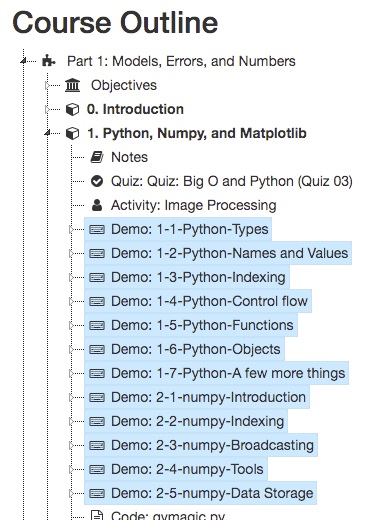
\includegraphics[height=0.5\textheight]{figures/L011/KloecknerPython.png}
    \caption{Recommended demos from Andreas Kloeckner's class site.}
    \label{fig0kloecknerSite}
\end{figure}

Also recommended are
\begin{itemize}
    \item PEP: The Python style guide \url{https://pep8.org}
    \item Flake8: An automatic Python style checker \url{http://flake8.pycqa.org/en/latest/}
\end{itemize}

%% TW: following can be achieved with \myvbox[mytermbg]{sudo apt-get install python3-numpy python3-scipy python3-matplotlib ipython3}
%\begin{tsession}{mytermbg}
%\begin{verbatim}
%sudo apt-get install python3-numpy python3-scipy python3-matplotlib ipython3
%\end{verbatim}
%\end{tsession}

%% use \texttt for command stuff. The apostrophes are not valid when pasted in python otherwise.
%print('Yellow world!')

%% link to something like this ? or other tutorial ? https://matplotlib.org/3.1.1/tutorials/introductory/sample_plots.html
